\documentclass[12pt]{article}

\usepackage{listings}
\usepackage{biblatex}



\usepackage{amssymb}
\usepackage{caption}

\usepackage{graphicx}
\usepackage{graphics}


\usepackage{amsmath}
\graphicspath{{/storage/self/primary/Download/latexnew/fig}}
\begin{document}

\begin{enumerate}
\item For the given digital circuit, $A = B = 1$. Assume that AND, OR, and NOT gates have propagation delays of $10\mathrm{ns}$,$10\mathrm{ns}$, and $5\mathrm{ns}$ respectively. All lines have zero
propagation delay. Given that $C = 1$ when the circuit is turned on, the frequency of steady-state oscillation of the output $Y$  is  \rule{30pt}{1pt}.

\hfill (GATE IN 2023)
\begin{figure}[!ht]
        \centering  
        
        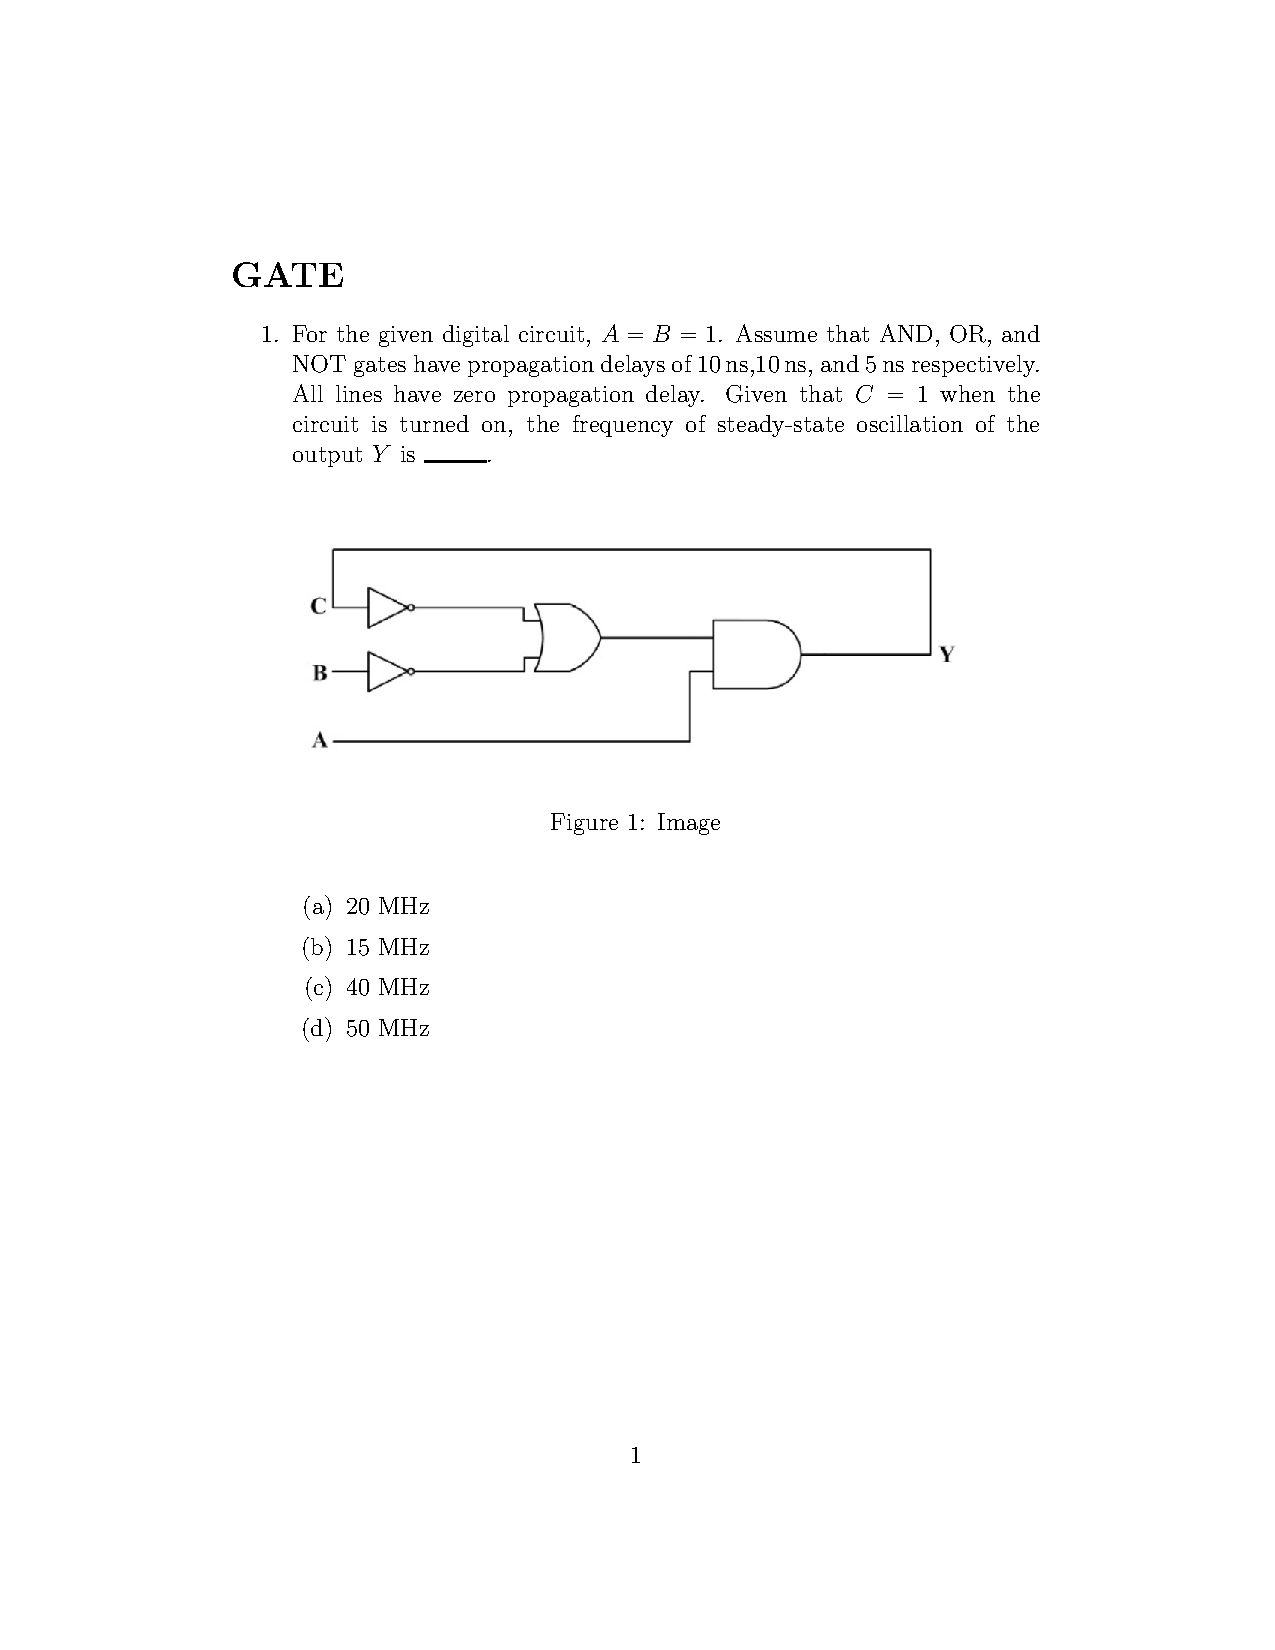
\includegraphics[width=\columnwidth]{/sdcard/digital-design/gate.png}
        \caption{Image}
        \label{fig:Image}
        
\end{figure}
    \begin{enumerate}
        \item $20 \mathrm{MHz}$
        \item $15 \mathrm{MHz}$
        \item $40 \mathrm{MHz}$
        \item $50 \mathrm{MHz}$
    \end{enumerate}
  \end{enumerate}
\end{document}
